\documentclass[12pt]{article}
\usepackage[a4paper]{geometry}
%\userpackage[top=1 in, bottom=1.25 in, left=1.1 in, rigth=1.1 in] {geometry}
%\usepackage[paperwidth=17cm, paperheight=22.5cm, bottom=2.5cm, right=2.5cm]{geometry}
\usepackage[utf8]{inputenc}
%\usepackage[a4paper, top=2.5cm, bottom=2.5cm, left=2.2cm, right=2.2cm]
%{geometry}
%\usepackage[myheadings]{fullpage}
\usepackage{fancyhdr}
\usepackage{lastpage}
%\usepackage{float}
\usepackage{graphicx, wrapfig, subcaption, setspace, booktabs}
\usepackage{graphicx}
\usepackage[T1]{fontenc}
\usepackage[font=small, labelfont=bf]{caption}
%\usepackage{fourier}
\usepackage[protrusion=true, expansion=true]{microtype}
\usepackage[english]{babel}
\usepackage{sectsty}
\usepackage{url, lipsum}
\usepackage[T1]{fontenc}
\usepackage{icomma}
\usepackage{siunitx}
\usepackage{ragged2e}
\usepackage{amsmath}
\usepackage{comment}
\usepackage{enumerate}
%\usepackage{changepage}
\usepackage{anysize}




\newcommand{\HRule}[1]{\rule{\linewidth}{#1}}
\onehalfspacing
\setcounter{tocdepth}{5}
\setcounter{secnumdepth}{5}

%-------------------------------------------------------------------------------
% HEADER & FOOTER
%-------------------------------------------------------------------------------


\begin{comment}
-Udledninger
$$
\begin{aligned}


\end{aligned}
$$

-Opgavetekst
\begin{figure}[H]
\includegraphics[width=0.5\textwidth]{"path"}
\end{figure} 


-Opgave billede med tekst
\begin{figure}[H]
\caption{"Billedtekst"}
\includegraphics[width=0.5\textwidth]{"path"}
\end{figure} 

-Værdier
$\\

$


\end{comment}
\begin{document}

\begin{titlepage}

\title{ \normalsize 
		%\begin{figure}
        \begin{center}
        
\includegraphics[height=6cm]{Logo.jpg}
        \end{center}
       % \end{figure}
        \LARGE \textsc{\textbf{Universidad De Sonora}} \\ \bigskip
		\Large División de Ciencias Exactas y Naturales \\
        Licenciatura En Física \\ \bigskip
        \bigskip
        Física Computacional I
		\\ [0.1cm]  
		\HRule{2pt} \\
		\Large \textbf{{Reporte de Actividad 5}} \\
        \textit{\textbf{"Preparando Datos con Ayuda de Emacs"}}
		\HRule{2pt} \\
		\normalsize \vspace*{0.001\baselineskip}}
        
\date{\bigskip \Large Hermosillo, Sonora  \hspace*{\fill}  Marzo 6 de 2018}

        
\author{
		\Large\textbf{ César Omar Ramírez Álvarez} \\ \bigskip
        \\ \bigskip
       \Large Profr. Carlos Lizárraga Celaya}
       \end{titlepage}
       \maketitle
       

\newpage
\pagestyle{plain}

\section*{Introdución}
Emacs es un editor de texto con una gran cantidad de funciones, muy popular entre programadores y usuarios técnicos. GNU Emacs es parte del proyecto GNU y la versión más popular de Emacs con una gran actividad en su desarrollo. El manual de GNU Emacs lo describe como "un editor extensible, personalizable, auto-documentado y de tiempo real."\\

En esta ocasión, con motivo de la práctica cinco en la que se propuso utilizar emacs para realizar limpieza y análisis de datos para después con el uso de jupyter dar una interpretación de los mismos, a través de gráficos. Los datos fueron obtenidos de los sondeos atmoféricos de la estación \textit{Camborne Observations} (mismos que fueron utilizados en actividades anteriores).\\

Datos clave con los que trabajaremos son los parámetros CAPE y PW que a lo largo del presente reporte daremos su definición física, además se presentará todo el procedimiento necesario para la limpieza y filtración de datos (lo mas entendible posible), así como el análisis realizado con Phyton y el apoyo de sus librerias. Por último, se presentarán los resultados obtenidos y las conclusiones correspndientes.

\section*{Fundamentos}
Para nuestro caso, nos interesa la relación entre CAPE y PW por lo que procederemos a definir estos parámteros:
\subsection*{CAPE}
\begin{wrapfigure}{l}{0.3\textwidth}
    \centering
    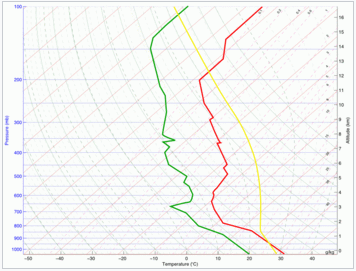
\includegraphics[width=0.3\textwidth]{CAPE.png}
\end{wrapfigure}
En meteorología, Convective Available Potential Energy (CAPE) hace referencia a la energía potencial disponible para la convección en un momento dado. Es energía por unidad de masa y no posee las medidas típicas de otros índices de inestabilidad, optando por la unidad de Joules/Kilogramos. Se trata de uno de los parámetros convectivos más interesantes de todos aquellos que se derivan de los modelos meteorológicos. Se trata de un parámetro que nos indica cuanta energía está disponible para la convección en caso de que esta se inicie.\\

Sus valores pueden ir entre 0 y unos pocos miles indicando un mayor grado de inestabilidad cuanto mayor es su valor, esta directamente relacionado con el máximo valor potencial de la velocidad vertical de las corrientes ascendentes, por tanto, valores mas altos indican un mayor potencial a tener un clima severo.

\subsection*{PW}
\begin{wrapfigure}{r}{0.3\textwidth}
    \centering
    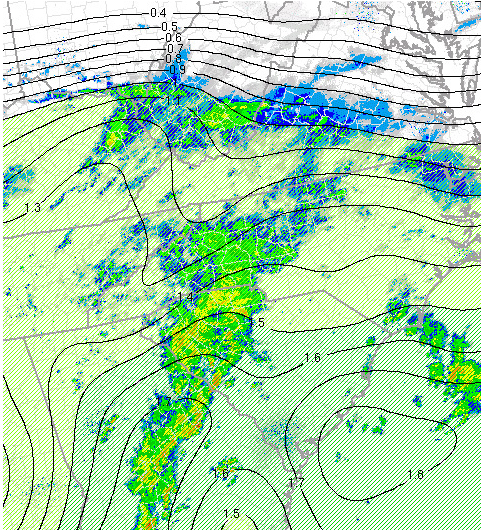
\includegraphics[width=0.3\textwidth]{PW.png}
\end{wrapfigure}
Precipitable Water (PW) "agua precipitable" es la cantidad de agua, expresada como altura o masa, que se obtendría si todo el vapor de agua contenido en una columna específica de la atmósfera, de sección transversal horizontal unitaria, se condensase y precipitase. Cabe reslatar que no indica cuanto va a llover.\\

El valor de Agua Precipitable también es un valor instantáneo de la cantidad de humedad en el aire sobre una ubicación. Puede precipitar más que la cantidad de valor precipitable, ya que puede ocurrir convergencia de humedad y la precipitación cae durante un lapso de tiempo y no es instantánea.
El valor de Agua Precipitable le da al pronosticador una idea de la cantidad de humedad en el aire. Los valores más altos indican una mayor disponibilidad de humedad para generar lluvia si se desarrolla precipitación.
 
\section*{Práctica}

\subsection*{Limpieza y Preparación de Datos}
Para realizar la limpieza de nuestros datos, la primera acción que se realizó fue tomar el creado y utilizado en la actividad anterior. El contenido de ese archivo son los registros de todos los meses del año de 2017 proporcionados pior la estación \textit{Camborne Observations}.\\

Con el apoyo de un script conteniendo el comando egrep dentro de él, se seleccionaron datos en específico, que para este caso fueron: los dos parámetros a analizar (CAPE y PW) y el número de la estación con la fecha de los lanzamientos realizados. El script al que llamamos "filtro" es el siguiente:
\begin{center}
	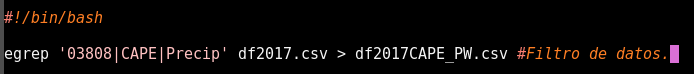
\includegraphics[height=1.5cm]{script.png}
\end{center}
Ejecutando el script se obtuvo el siguiente archivo df2017CAPE\_PW.csv, a continuación mostramos cierta parte de su contenido:
\begin{center}
	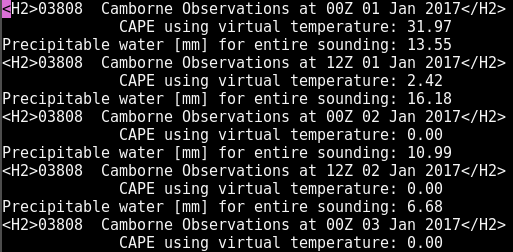
\includegraphics[height=6cm]{datoscompletos.png}
\end{center}
Ahora bien, se podria decir que aquí inica lo "bueno", pues para utilizar estos datos con la finalidad que se nos plantea en la actividad es necesario realizar una limpieza correspondiente, ya que como nos podemos percatar de las actividades pasadas cuando se hace uso de Jupyter para leer datos desde archivo, éste debe estar limpio, y con limpio hacemos referencia a que no debe haber texto presente y debe estar en columnas separados por comas. Gracias al uso de emacs y sus herramientas podemos realizar la limpieza del archivo generado siguiendo cierto procedimiento.\\

Como un primer paso es seleccionar el renglón de texto que tiene a la estación y su nombre evitando incluir el lanzamiento, esto anterior se realiza utilizando el comando Ctrl + space bar, una vez seleccionado se "corta" (como en Word), es decir, por medio del comando Ctrl + w se manda la linea seleccionada al junk donde se queda guardado. Posteriormente se "pega" si es el caso lo que cortamos con el comando Ctrl + y. Ahora bien, si lo que queremos es deshacernos de todos los renglones que contengan lo que ya tenemos seleccionado (en el documento se repite) es necesario regresarnos al inicio del archivo, esto se hace con ayuda del comando Ctrl + >, estando ahí se presiona la tecla Esc y posteriormente el \% y en la parte de abajo nos aparece una pregunta de que es lo que se quiere reemplazar, por lo que ahí pegamos con Ctrl + y y damos Enter (se pega lo que teniamos cortado), despues se nos pregunta con que deseamos reemplazarlo, como en esta ocasión solo queremos eliminarlo solo daremos Enter y para finalizar presionamos la tecla !. \\

Esto fue el tratamiento para la limpieza de los datos, se repitió varias veces hasta quedarnos con los datos en un solo renglón por cada lanzamiento, además sustituimos el espacio entre ellos por comas para tener ya bien organizadas las columnas y por último cambiamos el nombre de los meses por sus numeros que les corresponden. El archivo resultado fue el siguiente (una parte):
\begin{center}
	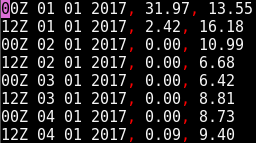
\includegraphics[height=4cm]{datos.png}
\end{center}
Como los lanzamientos son 2 por día, es necesario separar los datos debido a su lanzamiento, los lanzamientos estan clasificados mediante 00Z y 12Z. La separación se hace utilizando el cmando egrep que puede ser ejecutado desde la terminal o mediante un script.
\begin{center}
	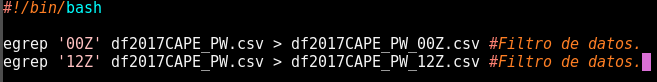
\includegraphics[height=1.5cm]{losscript.png}
\end{center}
Estos archivos aún contienen texto innecesario, por lo que procedemos a eliminarlo para que quede listo para su posterior análisis desde Jupyter Notebook. El archivo final es de la siguiente forma:
\begin{center}
	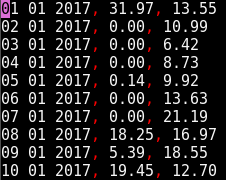
\includegraphics[height=4cm]{datosfinal.png} \hspace*{\fill}
    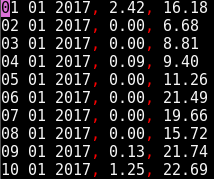
\includegraphics[height=4cm]{datosfinal2.png}
\end{center}

\subsection*{Análisis de Datos}
Desde nuestro Jupyter Notebook podemos leer los archivos por medio de la biblioteca de Pandas de Phyton como se ha trabajado en actividades anteriores, cabe resaltar que se agragaron todas las bibliotecas anteriores y una nueva "datetime" que es utilizada para dar formato de fecha a los datos.
\begin{center}
	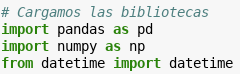
\includegraphics[height=1.9cm]{bibliotecas.png}
\end{center}
Ahora bien, colocamos los archivos en un dataframe y nombramos sus columnas, convirtiendo también el parámetro CAPE en numérico:
\begin{center}
	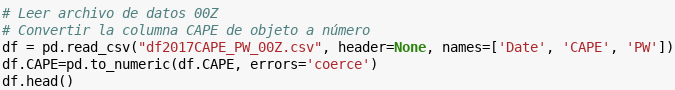
\includegraphics[height=2cm]{lectura.png}
    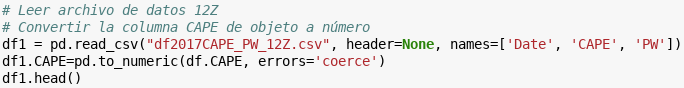
\includegraphics[height=1.91cm]{lectura2.png}
\end{center}
La fecha es de tipo objeto, por lo que la transformamos a tipo fecha con el apoyo de la biblioteca nueva que ingresamos:
\begin{center}
	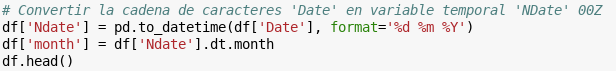
\includegraphics[height=1.81cm]{conversion.png}
    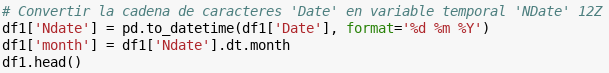
\includegraphics[height=1.91cm]{conversion1.png}
\end{center}
\begin{center}
	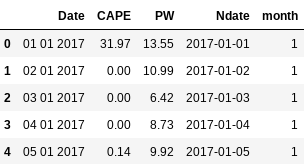
\includegraphics[height=4cm]{conversion0.png} \hspace*{\fill}
    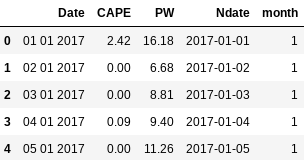
\includegraphics[height=4cm]{conversion01.png}
\end{center}
Teniendo ésto ya podemos realizar el análisis de los datos, en el caso de las gráficas obtenidas son de un nuevo tipo, las llamadas "box plot" y nos perimiten ver la relación que se cumple entre los datos, en esta ocasión mostraremos la relación que guardan CAPE y PW. Este tipo de gráficas también nos indica que tan sesgados estan los datos para saber si son correctos o no (refiriendonos a su toma). También se presentan gráficas que representan la regresión de los datos condicionados a su fecha. A continuación se presentan los códigos generadores correspondientes:
\begin{center}
	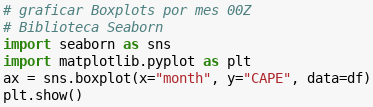
\includegraphics[height=2cm]{1.png} \hspace*{\fill}
    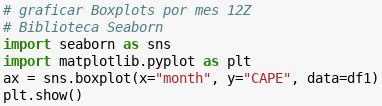
\includegraphics[height=2cm]{2.png}
\end{center}
\begin{center}
	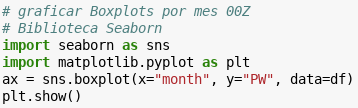
\includegraphics[height=2cm]{11.png} \hspace*{\fill}
    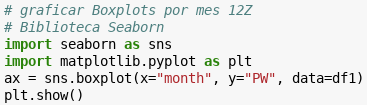
\includegraphics[height=2cm]{22.png}
\end{center}
\begin{center}
	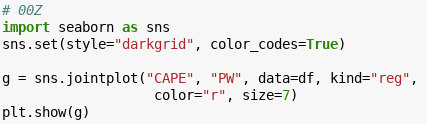
\includegraphics[height=2cm]{111.png} \hspace*{\fill}
    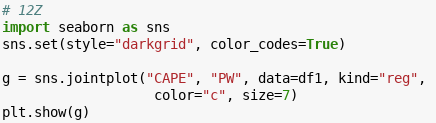
\includegraphics[height=2cm]{222.png}
\end{center}
\begin{center}
	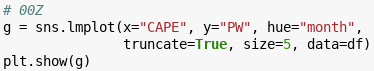
\includegraphics[height=1.5cm]{1111.png} \hspace*{\fill}
    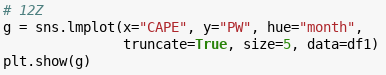
\includegraphics[height=1.5cm]{2222.png}
\end{center}
\section*{Resultados}
Primeramente tenemos el diagrama de caja del lanzamiento 00Z, la primera gáfica es del parámetro CAPE y la segunda de PW:
\begin{center}
	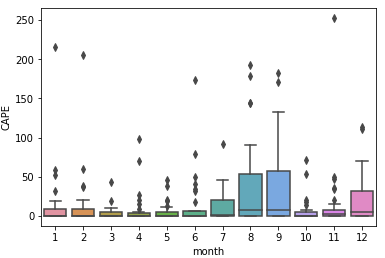
\includegraphics[height=5cm]{01.png} \hspace*{\fill}
    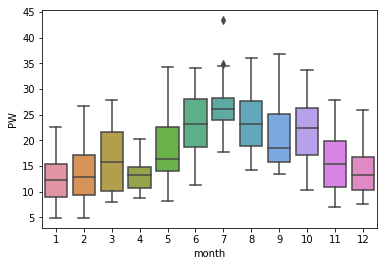
\includegraphics[height=5cm]{011.png}
\end{center}
Como podemos observar, en el caso de CAPE la mayoría de las veces es casi igual a cero, es decir las medidas de los datos están muy cerca de ese valor, y por ende las cajas también no estan. Esto se puede interpretar diciendo que la mayoría de los puntos están sesgados, es decir, por afuera de la caja. La que casi no presenta esto es la del mes de Septiembre. \\

Para el caso de PW, sucede casi lo contrario, pues las cajas estan alejadas del cero y sus puntos estan sesgados (excepto en el mes de Julio). Podemos notar que en veranos es cunado se presenta más, decayendo en invierno.\\

Ahora presentamos el diagrama del lanzamiento 12Z, la primera gáfica es del parámetro CAPE y la segunda de PW:

\begin{center}
	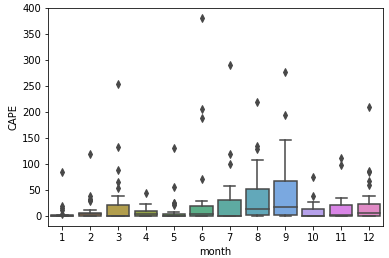
\includegraphics[height=5cm]{02.png} \hspace*{\fill}
    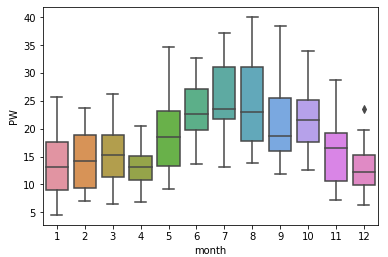
\includegraphics[height=5cm]{022.png}
\end{center}
De aqui podemos observar, en el caso de CAPE, al igual que en el caso anterior la mayoria de las veces se tiende a cero, teniendo las medidas muy cercanas a ese valor y por ende las cajas también, pero es muy notorio ahora que ahora se tiene mas puntos sesgados.\\

Tomando en cuenta el caso de PW, las cajas se encuentra mas alejadas del cero y solo cuentan con un punto de sesgo en el mes de Diciembre, aunque se mantenga el echo de que en verano existan valores más altos, comparados con la anterior (00Z) son valores aun mas grandes.\\

A continuación tenemos las gráficas que presentan la distribución de los datos como parámetros separados y como uno en función del otro, para ver que relación guardan, la primera de ellas es la correspondiente a 00Z y la segunda a 12Z.
\begin{center}
	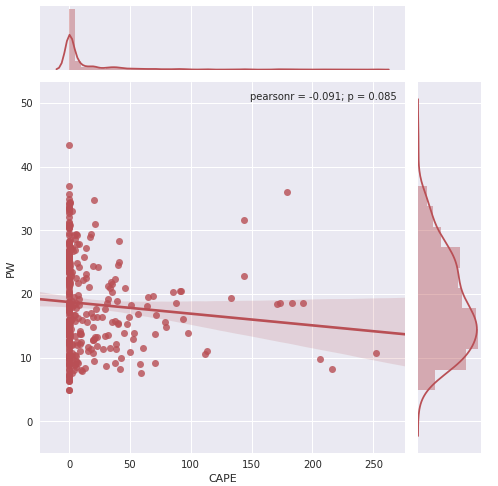
\includegraphics[height=7cm]{0111.png} \hspace*{\fill}
    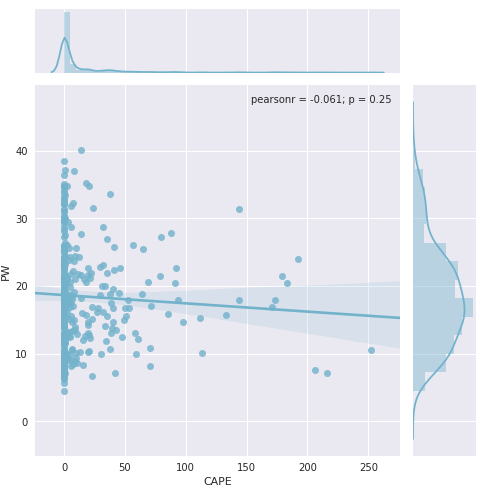
\includegraphics[height=7cm]{0222.png}
\end{center}
En cada una de los dos diagramas anteriores existen tres gráficas, la gráfica de la parte de arriba pertenece a la distribución de CAPE conforme pasan los días y la gráfica lateral hace referencia a la distribución de PW conforme pasan los días tambien, mientras que la gráfica central (la más grande) es el ajuste en la relación de los dos parámetros.\\

Podemos notar que para ambos lanzamientos las gráficas de arriba y las laterales son muy parecidas, mientras que las centrales difieren un poco en la recta del ajuste. El indicador $p$ muestra que tan relacionados estan los datos de cada una de las gráficas gráficas, es notorio que es un valor alto comparado con el coeficiente de correlación, por lo que se podria decir que hablamos de una relación lineal entre los datos.\\

Por último, se presentan las graficas de la relación de los parámetros a lo largo del año:
\begin{center}
	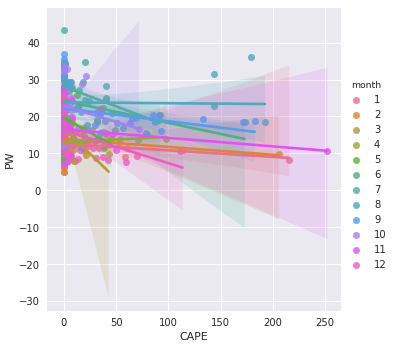
\includegraphics[height=6cm]{01111.png} \hspace*{\fill}
    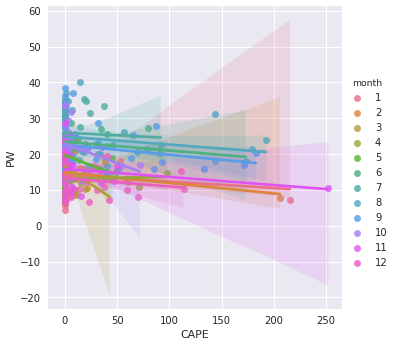
\includegraphics[height=6cm]{02222.png}
\end{center}
Para cada mes se observa que se genera una recta y dependiendo del cambio entre los datos (CAPE y PW) el triángulo formado cambia de posiciones. Éstos triángulos representan la distribución que tiene los datos cada mes. Es notorio que en ambos lanzamientos tenemos triángulos hacia arriba y hacia abajo por lo que podemos decir que si existe cierta relación lineal entre ambos parámetros.

\section*{Conclusión}
En actividades anteriores se habia mencionado que la limpieza de datos es un proceso que implica más tiempo y experiencia para tener un buen realizar análisis de los mismos, como parte de la actividad propuesta nos dimos cuenta de eso, es muy importante tener bien organizados los datos antes del proceso de análisi. Sin duda el apoyo de emacs para esta práctica nos perimitó hacer la limpieza de una manera mas rápida y eficaz, con la ayuda de sus herrmaientas y comandos. Por último, la vista gráfica de los datos nos hacen reflexionar del comportamiento que se tiene, además con el ingreso de una nueva forma de gráficas complementa lo aprendido y da una nueva vista de ver datos cuando implican datos estadistico y de correlación entre parámetros.

\section*{Bibliografía}
\begin{itemize}
\item Agua precipitable. (2018). Aguamarket.com.  Recuperado el 4 de Marzo de 2018, desde http://www.aguamarket.com/diccionario/terminos.asp?Id=4550
\item  CAPE y algunas nociones básicas sobre convección atmosférica. (2018).\\ Meteoillesbalears.com.  Recuperado el 4 de Marzo de 2018, desde \\ http://www.meteoillesbalears.com/?p=623
\item  Emacs. (2018). Es.wikipedia.org.  Recuperado el 4 de Marzo de 2018, desde https://es.wikipedia.org/wiki/Emacs
\item  WHAT IS PRECIPITABLE WATER?. (2018). Theweatherprediction.com.\\ Recuperado el 4 de Marzo de 2018, desde\\ http://www.theweatherprediction.com/habyhints3/899/
\end{itemize}
\section*{Apéndice}
\begin{enumerate}
\item ¿Cómo se te hizo esta actividad? ¿Compleja, Difícil, Sencilla?\\
\textit{Primeramente se me hizo difícil, pues no sabia como usar emacs y sus comandos, ya que son diferentes a los utilizados en Word. Pero gracias a una actividad dinámica simple propuesta por el profesor me fui familiarizando con emacs.}

\item ¿Qué te llamó más la atención?\\
\textit{Lo fácil y rápido que es limpiar y seleccionar grandes cantidades datos con emacs, no me hubiera imaginado hacerlo manual.}

\item ¿Qué parte fue la que menos te interesó hacer?\\
\textit{En sí, todo me interesó, considero que fue algo introductorio (fácil) y que después aprenderemos mas cosas nuevas.}

\item ¿Cómo mejorarías esta actividad? ¿Qué le faltó? ¿Qué sobró?\\
\textit{El tiempo fue muy merecido para terminar la actividad, aunque me hubiera gustado una muy buena explicación de las gráficas reproducidas, ya que aunque eran fáciles de hacer, no teníal el contexto necesario para comprender lo que me estaban representando.}

\item ¿Hasta este punto, que te parece el uso de Jupyter para programar en Python? \\
\textit{En cada actividad me soprende más, pues posee grandiosas bibliotecas que nos apoyan en la parte gráfica, además es fácil de tratar y como nuevo recurso aprendimos una nueva forma de graficar.}

\end{enumerate}
\end{document}
